%\section{Exercises Part 1}

\subsection{Exercise 1.1: Sorting Complexity}
\textbf{Problem:} A sorting method with “Big-Oh” complexity $O(n \log n)$ spends exactly 1 millisecond to sort 1,000 data items. Given this, estimate how long it will take to sort 1,000,000 items.

\vspace{0.5em}
\textbf{Solution Steps:}
\begin{enumerate}[leftmargin=*,noitemsep]
    \item Understand the Problem: You need to find out how long it will take to sort 1,000,000 items using the given complexity.
    \item Identify Known Values:
    \begin{itemize}
        \item $T(1,000) = 1ms$
        \item Complexity is $O(n \log n)$
    \end{itemize}
    \item Calculate Constant $c$:
    \begin{itemize}
        \item Formula: $T(n) = c \cdot n \log n$
        \item Use $T(1,000) = 1ms$ to find $c$:
        \[ c = \frac{1ms}{1,000 \log 1,000} \]
    \end{itemize}
    \item Calculate $T(1,000,000)$:
    \begin{itemize}
        \item Use the formula $T(n) = c \cdot n \log n$
        \item Substitute $n = 1,000,000$:
        \[ T(1,000,000) = c \cdot 1,000,000 \cdot \log 1,000,000 \]
    \end{itemize}
    \item Simplify the Expression:
    \begin{itemize}
        \item Calculate $\log 1,000,000$
        \item Multiply and simplify to find the time in seconds.
    \end{itemize}
\end{enumerate}

\textbf{Exam Note:} Remember that $O(n \log n)$ complexity means the time increases logarithmically with the size of the data.

\textbf{Hint:} To solve similar exercises, focus on understanding the relationship between the given complexity and the time it takes to process a certain amount of data. Use the formula $T(n) = c \cdot f(n)$ to calculate the constant $c$ and then use it to find the time for a different amount of data.

\subsection{Exercise 1.2: Quadratic Algorithm}
\textbf{Problem:} A quadratic algorithm with processing time $T(n) = cn^2$ spends 1ms for 100 items. Calculate the time for 5,000 items.

\vspace{0.5em}
\textbf{Solution Steps:}
\begin{enumerate}[leftmargin=*,noitemsep]
    \item Understand the Problem: You need to calculate the time for 5,000 items given the complexity.
    \item Identify Known Values:
    \begin{itemize}
        \item $T(100) = 1ms$
        \item Complexity is $O(n^2)$
    \end{itemize}
    \item Calculate Constant $c$:
    \begin{itemize}
        \item Formula: $T(n) = c \cdot n^2$
        \item Use $T(100) = 1ms$ to find $c$:
        \[ c = \frac{1ms}{100^2} \]
    \end{itemize}
    \item Calculate $T(5,000)$:
    \begin{itemize}
        \item Use the formula $T(n) = c \cdot n^2$
        \item Substitute $n = 5,000$:
        \[ T(5,000) = c \cdot (5,000)^2 \]
    \end{itemize}
    \item Simplify the Expression:
    \begin{itemize}
        \item Calculate $(5,000)^2$
        \item Multiply and simplify to find the time in milliseconds.
    \end{itemize}
\end{enumerate}

\textbf{Exam Note:} Quadratic complexity $O(n^2)$ means time increases with the square of the data size.

\textbf{Hint:} To solve similar exercises, focus on understanding the relationship between the given complexity and the time it takes to process a certain amount of data. Use the formula $T(n) = c \cdot f(n)$ to calculate the constant $c$ and then use it to find the time for a different amount of data.

\FloatBarrier

\begin{table}[h]
    \centering
    \small
    \begin{tabularx}{\linewidth}{|X|X|X|}
        \hline
        Expression & Dominant term(s) & $O(\ldots)$ \\
        \hline
        5 + 0.001$n^3$ + 0.025$n$ & 0.001$n^3$ & $O(n^3)$ \\
        \hline
        500$n$ + 100$n^{1.5}$ + 50$n \log_{10} n$ & 100$n^{1.5}$ & $O(n^{1.5})$ \\
        \hline
        0.3$n$ + 5$n^{1.5}$ + 2.5 $\cdot$ $n^{1.75}$ & 2.5$n^{1.75}$ & $O(n^{1.75})$ \\
        \hline
        $n^2 \log_2 n$ + $n(n \log n)^2$ & $n^2 \log n$ & $O(n^2 \log n)$ \\
        \hline
        $n \log_3 n$ + $n \log_2 n$ & $n \log_3 n, n \log_2 n$ & $O(n \log n)$ \\
        \hline
        3 $\log_8 n$ + $\log_2 \log_2 \log_2 n$ & 3 $\log_8 n$ & $O(\log n)$ \\
        \hline
        100$n$ + 0.01$n^2$ & 0.01$n^2$ & $O(n^2)$ \\
        \hline
        0.01$n$ + 100$n^2$ & 100$n^2$ & $O(n^2)$ \\
        \hline
        2$n$ + $n^{0.5}$ + 0.5$n^{1.25}$ & 0.5$n^{1.25}$ & $O(n^{1.25})$ \\
        \hline
        0.01$n \log_2 n$ + $n(\log_2 n)^2$ & $n(\log_2 n)^2$ & $O(n(\log n)^2)$ \\
        \hline
        100$n \log_3 n$ + $n^3$ + 100$n$ & $n^3$ & $O(n^3)$ \\
        \hline
        0.003 $\log_4 n$ + $\log_2 \log_2 n$ & 0.003 $\log_4 n$ & $O(\log n)$ \\
        \hline
    \end{tabularx}
    \caption{Dominant terms and Big-Oh notation for various expressions.}
\end{table}

\begin{table}[h]
    \centering
    \small
    \begin{tabularx}{\linewidth}{|X|X|X|}
        \hline
        Statement & Is it TRUE or FALSE? & If it is FALSE then write the correct formula \\
        \hline
        Rule of sums: $O(f + g) = O(f) + O(g)$ & FALSE & $O(f + g) = \max\{O(f), O(g)\}$ \\
        \hline
        Rule of products: $O(f \cdot g) = O(f) \cdot O(g)$ & TRUE & \\
        \hline
        Transitivity: if $g = O(f)$ and $h = O(f)$ then $g = O(h)$ & FALSE & if $g = O(f)$ and $f = O(h)$ then $g = O(h)$ \\
        \hline
        $5n + 8n^2 + 100n^3 = O(n^4)$ & TRUE & \\
        \hline
        $5n + 8n^2 + 100n^3 = O(n^2 \log n)$ & FALSE & $5n + 8n^2 + 100n^3 = O(n^3)$ \\
        \hline
    \end{tabularx}
    \caption{Evaluation of Big-Oh notation statements.}
\end{table}

\begin{figure}[H]
    \centering
    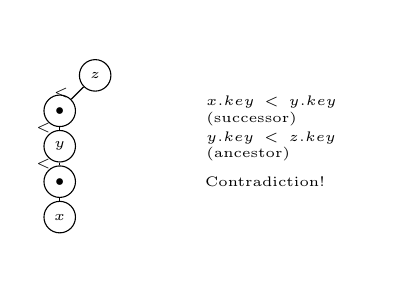
\begin{tikzpicture}[scale=0.45,
        level distance=1cm,
        level 1/.style={sibling distance=2cm},
        level 2/.style={sibling distance=1cm},
        every node/.style={circle,draw,inner sep=1pt,font=\tiny,minimum size=0.4cm}]
        
        % The tree showing contradiction
        \node (z) {$z$}
            child {
                node (leftz) {$\bullet$}
                child {
                    node (y) {$y$} 
                    child {
                        node (lefty) {$\bullet$}
                        child {
                            node (x) {$x$}
                        }
                        edge from parent node[left,draw=none,font=\tiny] {$<$}
                    }
                    edge from parent node[left,draw=none,font=\tiny] {$<$}
                }
                edge from parent node[left,draw=none,font=\tiny] {$<$}
            }
            child[missing];
            
        % Add explanatory text
        \node[draw=none,font=\tiny,text width=2cm,anchor=west] at (3,-1) 
            {$x.key < y.key$ (successor)};
        \node[draw=none,font=\tiny,text width=2cm,anchor=west] at (3,-2) 
            {$y.key < z.key$ (ancestor)};
        \node[draw=none,font=\tiny,text width=2cm,anchor=west] at (3,-3) 
            {Contradiction!};
    \end{tikzpicture}
    \caption*{\footnotesize Contradiction in BST property}
\end{figure}

\begin{figure}[H]
    \centering
    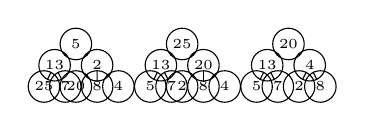
\begin{tikzpicture}[scale=0.45,
        level distance=0.6cm,
        level 1/.style={sibling distance=1.2cm},
        level 2/.style={sibling distance=0.6cm},
        level 3/.style={sibling distance=0.8cm},
        every node/.style={circle,draw,inner sep=1pt,font=\tiny,minimum size=0.4cm}]
        
        % Initial tree
        \node {5}
            child {node {13}
                child {node {25}}
                child {node {7}}
            }
            child {node {2}
                child {node {20}}
                child {node {8}}
                child {node {4}}
            };
            
        % After BUILD-MAX-HEAP
        \begin{scope}[xshift=3cm]
        \node {25}
            child {node {13}
                child {node {5}}
                child {node {7}}
            }
            child {node {20}
                child {node {2}}
                child {node {8}}
                child {node {4}}
            };
        \end{scope}
        
        % After first extraction
        \begin{scope}[xshift=6cm]
        \node {20}
            child {node {13}
                child {node {5}}
                child {node {7}}
            }
            child {node {4}
                child {node {2}}
                child {node {8}}
            };
        \end{scope}
    \end{tikzpicture}
    \caption*{\footnotesize HEAPSORT steps: Initial $\rightarrow$ BUILD-MAX-HEAP $\rightarrow$ First extraction}
\end{figure}

\sloppy
